% Slide 43: Anomaly Detection
\begin{frame}{مقدمه‌ای بر تشخیص ناهنجاری}{\lr{Anomaly Detection / Outlier Detection}}
  \begin{itemize}
    \setlength{\itemsep}{6pt}
    \item همچنین تحت عنوان \textbf{تشخیص داده‌های پرت \lr{(Outlier Detection)}} شناخته می‌شود.
    \item \textbf{هدف:} شناسایی خودکار نمونه‌های داده‌ای که به هر نحوی رفتاری کاملاً متمایز و نامتعارف نسبت به سایر داده‌ها دارند.
    \item \textbf{فرض بنیادی کار:}
    \begin{itemize}
      \item تعداد مشاهدات «عادی» در داده‌ها \textbf{بسیار بیشتر} از مشاهدات «غیرعادی» (ناهنجاری‌ها/پرت‌ها) است.
    \end{itemize}
    \item \textbf{دسته‌بندی روش‌های اصلی:}
    \begin{itemize}
      \setlength{\itemsep}{2pt}
      \item رویکردهای آماری \lr{(Statistical Approaches)}: نظیر \lr{IQR} و \lr{MAD}
      \item رویکردهای مبتنی بر فاصله \lr{(Distance-based Approaches)}
      \item رویکردهای مبتنی بر چگالی \lr{(Density-based Approaches)}
      \item رویکردهای مبتنی بر خوشه‌بندی \lr{(Clustering-based Approaches)}
    \end{itemize}
  \end{itemize}
\end{frame}

% Slide 44: Pipeline
\begin{frame}{جایگاه تشخیص ناهنجاری در خط لوله داده‌کاوی}{\lr{Anomaly Detection in the Data Mining Pipeline}}
  \begin{columns}[T]
    \begin{column}{0.54\textwidth}
      \begin{itemize}
        \setlength{\itemsep}{6pt}
        \item \textbf{کاربرد در خط لوله:} \lr{(Pipeline)}
        \begin{itemize}
          \setlength{\itemsep}{3pt}
          \item شناسایی و حذف داده‌های پرت از \textbf{مجموعه آموزش \lr{(Training Set)}} به منظور جلوگیری از انحراف مدل.
          \item حفظ داده‌های پرت در \textbf{مجموعه آزمون \lr{(Test Set)}} بدون تغییر، تا عملکرد مدل در شرایط دنیای واقعی محک بخورد.
        \end{itemize}
        \item تفکیک ناهنجاری واقعی از خطای ثبت حسگرها یا ورود داده.
      \end{itemize}
    \end{column}
    \begin{column}{0.44\textwidth}
      \begin{center}
        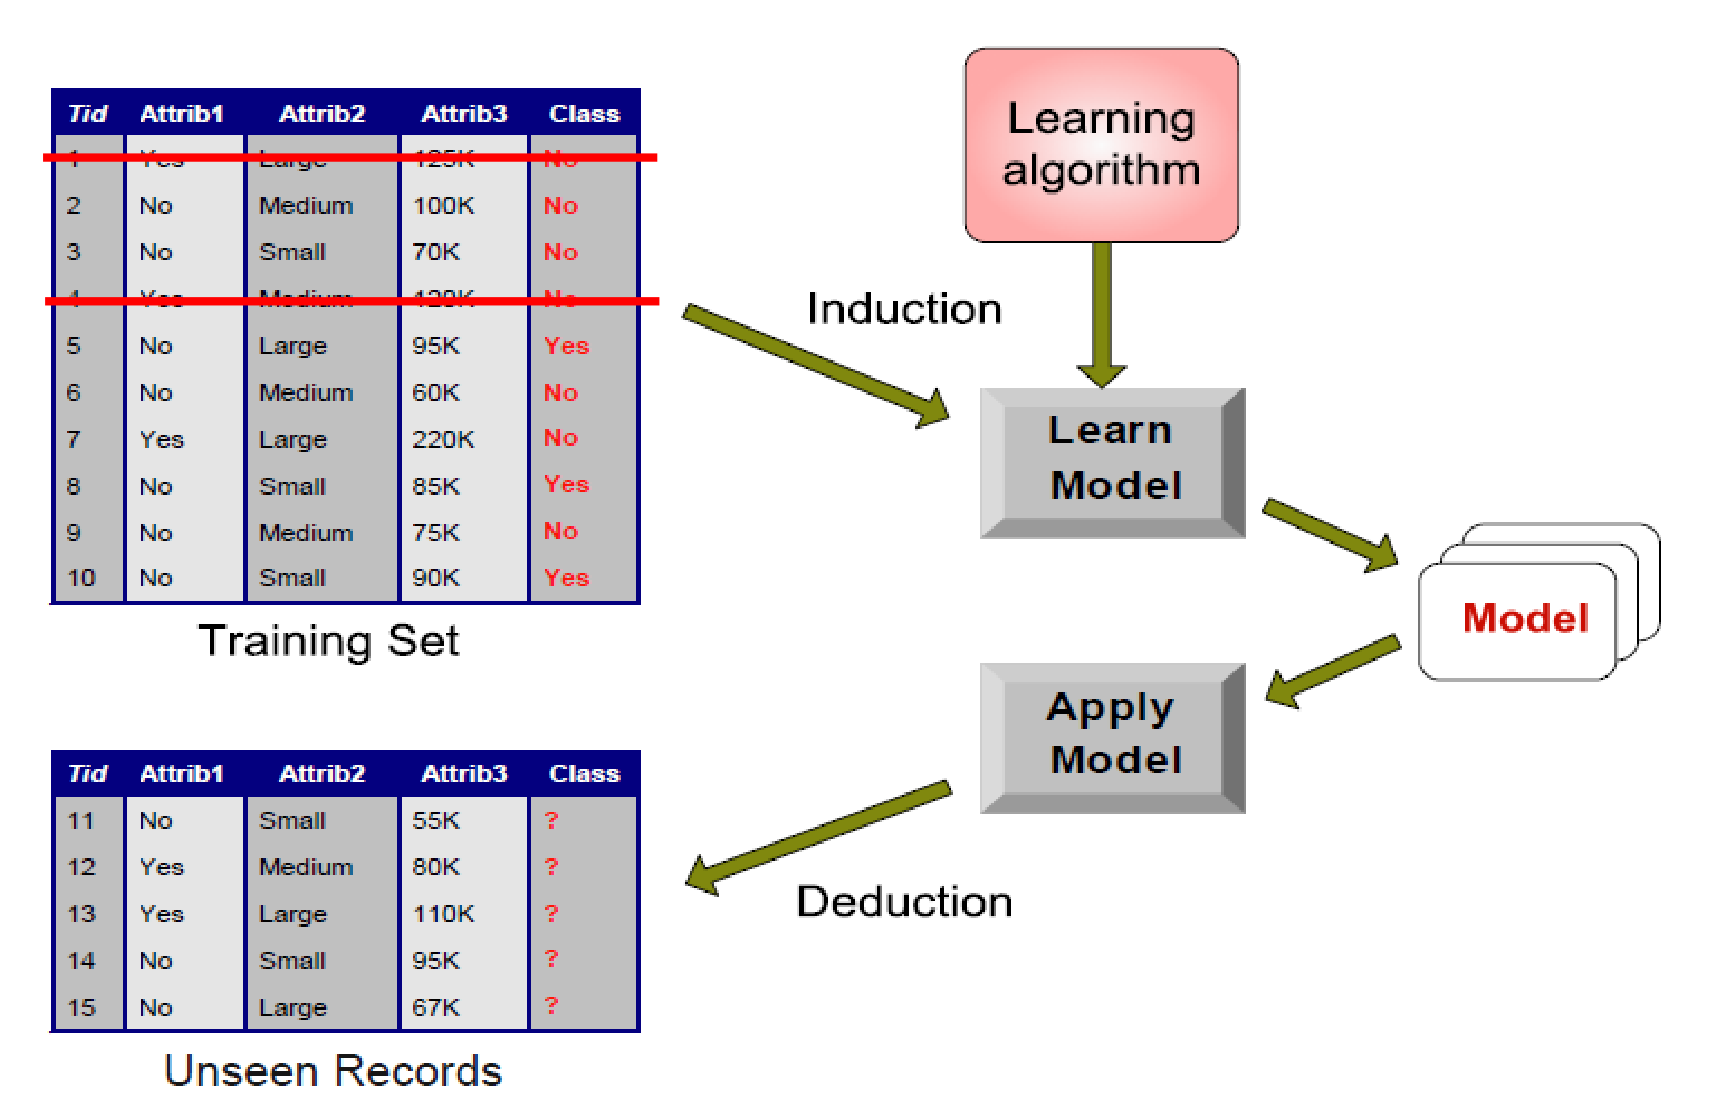
\includegraphics[width=\textwidth,height=4.5cm,keepaspectratio]{images/slide44_anomaly_pipeline.png}
      \end{center}
    \end{column}
  \end{columns}
\end{frame}

% Slide 45: Statistical Approaches
\begin{frame}{رویکردهای آماری تشخیص ناهنجاری}{\lr{Statistical Approaches to Outlier Detection}}
  \begin{columns}[T]
    \begin{column}{0.55\textwidth}
      \begin{itemize}
        \setlength{\itemsep}{5pt}
        \item فرض یک مدل پارامتریک برای توصیف توزیع داده‌ها (مانند توزیع نرمال یا گاوسی).
        \item اعمال آزمون‌های آماری که به عوامل زیر بستگی دارند:
        \begin{itemize}
          \setlength{\itemsep}{3pt}
          \item نوع توزیع آماری داده‌ها \lr{(Data Distribution)}.
          \item پارامترهای توزیع (مانند میانگین $\mu$ و واریانس $\sigma^2$).
          \item تعداد مورد انتظار داده‌های پرت یا سطح اطمینان \lr{(Confidence Limit)}.
        \end{itemize}
        \item داده‌هایی که احتمال وقوع آن‌ها تحت توزیع مفروض بسیار ناچیز است، به عنوان ناهنجاری علامت‌گذاری می‌شوند.
      \end{itemize}
    \end{column}
    \begin{column}{0.42\textwidth}
      \begin{center}
        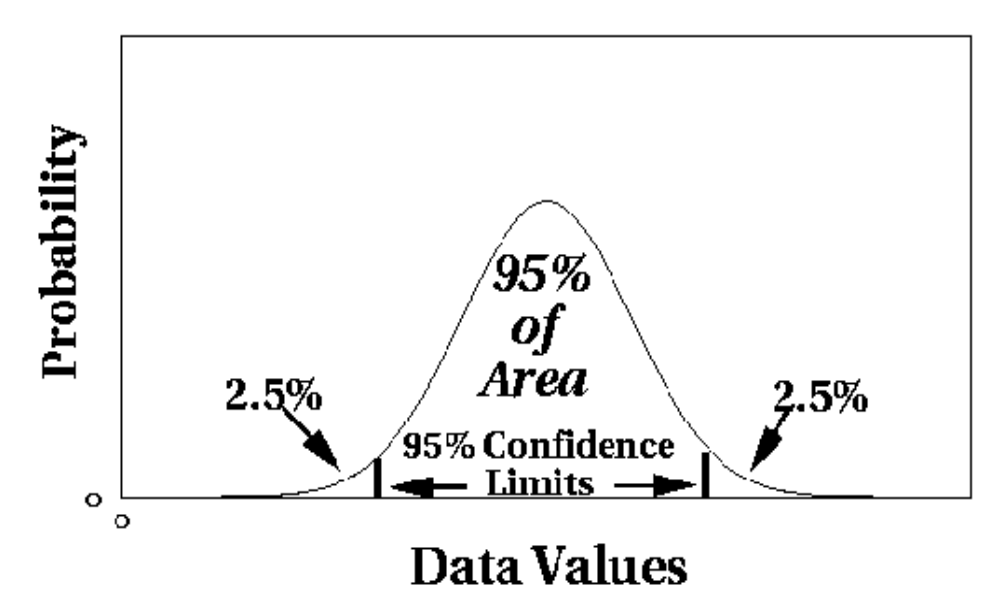
\includegraphics[width=\textwidth,height=4.2cm,keepaspectratio]{images/slide45_grubbs_normal_curve.png}
      \end{center}
    \end{column}
  \end{columns}
\end{frame}

% Slide 46: IQR
\begin{frame}{دامنه میان‌چارکی (\lr{IQR})}{\lr{Interquartile Range (IQR)}}
  \begin{columns}[T]
    \begin{column}{0.56\textwidth}
      {\fontsize{7.8}{10}\selectfont
      \setlength{\abovedisplayskip}{2pt}
      \setlength{\belowdisplayskip}{2pt}
      \begin{itemize}
        \setlength{\itemsep}{1pt}
        \item تقسیم داده‌ها به ۴ چارک آماری (با فرض توزیع نرمال):
        \begin{itemize}
          \setlength{\itemsep}{1pt}
          \item $Q_1$: برای $\%75$ داده‌ها رابطه $x \ge Q_1$ برقرار است.
          \item $Q_3$: برای $\%25$ داده‌ها رابطه $x \ge Q_3$ برقرار است.
          \item $\text{IQR} = Q_3 - Q_1$
        \end{itemize}
        \item \textbf{قاعده تشخیص دادۀ پرت:} هر داده خارج از بازه:
        \[
          [Q_1 - 1.5 \times \text{IQR} \ , \ Q_3 + 1.5 \times \text{IQR}]
        \]
        \item \textbf{مثال عددی:}
        \begin{itemize}
          \setlength{\itemsep}{1pt}
          \item داده‌ها: $\{0, 1, 1, 3, 3, 5, 7, 42\}$
          \item میانه $=3$، $Q_1=1$، $Q_3=7$ $\Rightarrow \text{IQR} = 6$
          \item بازه مجاز: $[1 - 1.5(6) \ , \ 7 + 1.5(6)] = [-8, 16]$
          \item عدد $\mathbf{42}$ خارج از بازه است $\Rightarrow$ \textbf{داده پرت}.
        \end{itemize}
      \end{itemize}
      }
    \end{column}
    \begin{column}{0.42\textwidth}
      \begin{center}
        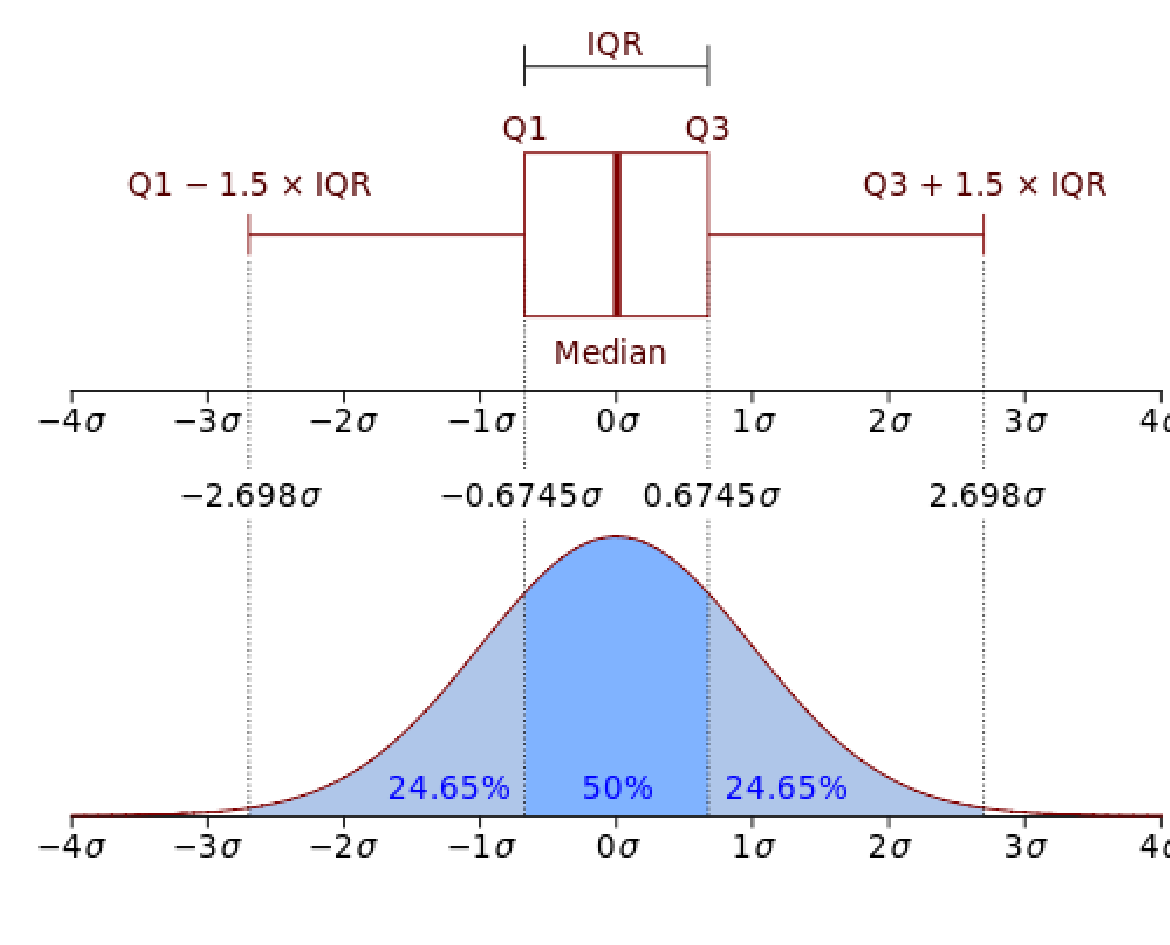
\includegraphics[width=\textwidth,height=4.5cm,keepaspectratio]{images/slide46_iqr_boxplot.png}
      \end{center}
    \end{column}
  \end{columns}
\end{frame}

% Slide 47: MAD
\begin{frame}{معیار انحراف مطلق از میانه (\lr{MAD})}{\lr{Median Absolute Deviation (MAD)}}
  \begin{itemize}
    \setlength{\itemsep}{2pt}
    \item \textbf{تعریف:} \lr{MAD} میانه قدرمطلق انحراف داده‌ها از میانه نمونه:
  \end{itemize}
  \[
    \tilde{X} = \text{median}(X), \quad \text{MAD} = \text{median}(|X_i - \tilde{X}|)
  \]
  \begin{columns}[T]
    \begin{column}{0.65\textwidth}
      \begin{itemize}
        \setlength{\itemsep}{2pt}
        \item داده‌هایی با فاصله بیش از $k \times \text{MAD}$ از میانه، پرت محسوب می‌شوند (معمولاً $k=3$).
        \item \textbf{مثال عددی:}
        \begin{itemize}
          \item داده‌ها: $X = \{0, 1, 1, 3, 5, 7, 42\} \Rightarrow \tilde{X} = 3$
          \item قدرمطلق انحرافات: $\{3, 2, 2, 0, 2, 4, 39\}$
          \item انحرافات مرتب‌شده: $\{0, 2, 2, \mathbf{2}, 3, 4, 39\} \Rightarrow \text{MAD} = 2$
          \item بازه مجاز: $[3 - 3(2) \ , \ 3 + 3(2)] = [-3, 9]$
          \item عدد $\mathbf{42}$ خارج از بازه است $\Rightarrow$ \textbf{داده پرت}.
        \end{itemize}
      \end{itemize}
    \end{column}
    \begin{column}{0.32\textwidth}
      \begin{center}
        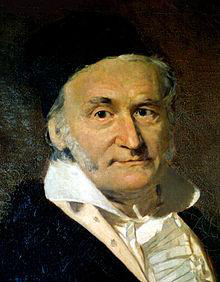
\includegraphics[width=0.72\textwidth,height=3.0cm,keepaspectratio]{images/slide47_gauss_original.png}\\[0.05cm]
        {\fontsize{7.5}{9}\selectfont\color{mannheimblue}\lr{\textbf{Carl Friedrich Gauss}}}\\[0.02cm]
        {\fontsize{6.8}{8}\selectfont\color{gray}\lr{1777--1855}}
      \end{center}
    \end{column}
  \end{columns}
\end{frame}

% Slide 48: Outliers vs Extreme Values
\begin{frame}{داده‌های پرت در برابر مقادیر فرین}{\lr{Outliers vs. Extreme Values}}
  \begin{itemize}
    \setlength{\itemsep}{4pt}
    \item تا اینجا فقط مقادیر فرین و کرانه‌ای \lr{(Extreme Values)} را بررسی کردیم.
    \item اما داده‌های پرت می‌توانند در \textbf{نواحی میانی یا غیرفرین} نیز رخ دهند!
    \item در این شرایط روش‌های متکی بر دامنه نظیر \lr{IQR} شکست می‌خورند:
    \begin{itemize}
      \setlength{\itemsep}{2pt}
      \item در مثال زیر: میانه $0$ است، $Q_1=-1, Q_3=1 \Rightarrow \text{IQR}=2$.
      \item بازه مجاز: $[-4, +4]$ $\Rightarrow$ هیچ نقطه‌ای به عنوان پرت شناخته نمی‌شود، در حالی که نقاط جداافتاده آشکاری وجود دارند!
    \end{itemize}
  \end{itemize}
  \vspace{0.3cm}
  \begin{center}
    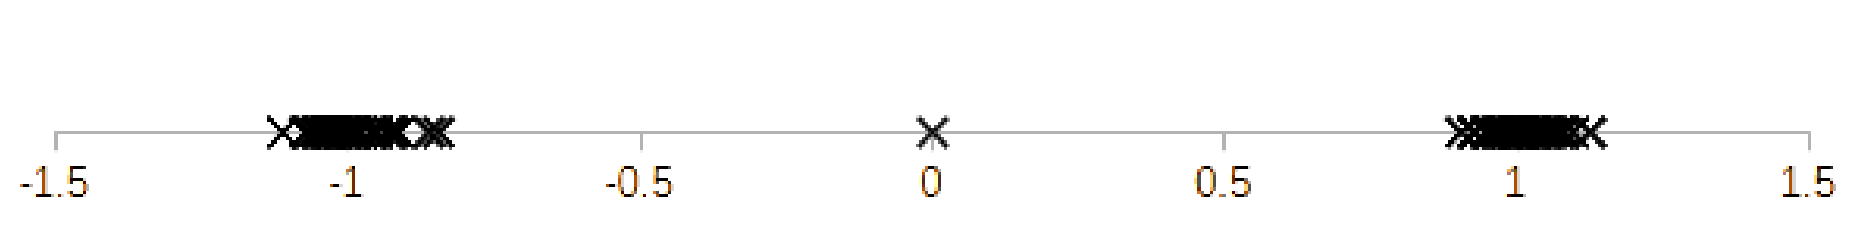
\includegraphics[width=0.88\textwidth,height=1.8cm,keepaspectratio]{images/slide48_outliers_vs_extremes.png}
  \end{center}
\end{frame}

% Slide 49: Distance-based Approaches
\begin{frame}{رویکردهای مبتنی بر فاصله}{\lr{Distance-based Approaches}}
  \begin{columns}[T]
    \begin{column}{0.65\textwidth}
      \textbf{روش‌های مبتنی بر نزدیک‌ترین همسایه‌ها}: \lr{(Nearest-Neighbor)}
      \begin{itemize}
        \setlength{\itemsep}{4pt}
        \item محاسبه فواصل دوبه‌دوی تمام نقاط داده در فضا.
        \item \textbf{تعاریف گوناگون برای دادۀ پرت:}
        \begin{enumerate}
          \setlength{\itemsep}{3pt}
          \item نقاطی که کمتر از $p$ همسایه در فاصله $D$ از آن‌ها وجود دارد.
          \item تعداد $n$ نقطه برتر که فاصله آن‌ها تا \textbf{$k$-امین نزدیک‌ترین همسایه} بیشترین مقدار است.
          \item تعداد $n$ نقطه برتر که \textbf{میانگین فاصله} آن‌ها تا $k$ نزدیک‌ترین همسایه بیشترین مقدار است.
        \end{enumerate}
      \end{itemize}
    \end{column}
    \begin{column}{0.32\textwidth}
      \begin{center}
        \vspace*{0.3cm}
        \fcolorbox{mannheimblue}{codebg}{%
          \begin{minipage}{0.92\textwidth}
            \centering
            \vspace*{0.15cm}
            {\fontsize{8.5}{11}\selectfont\textbf{بسته پایتون}}\\[0.15cm]
            {\fontsize{13}{16}\selectfont\textbf{\lr{PyOD}}}\\[0.1cm]
            {\scriptsize\lr{Python Outlier Detection}}\\[0.15cm]
            {\tiny شامل انواع روش‌های فاصله‌ای، زاویه‌ای و مبتنی بر همسایگی}
            \vspace*{0.15cm}
          \end{minipage}%
        }
      \end{center}
    \end{column}
  \end{columns}
\end{frame}
